\documentclass{VUMIFInfKursinis}
\usepackage{algorithmicx}
\usepackage{algorithm}
\usepackage{algpseudocode}
\usepackage{amsfonts}
\usepackage{amsmath}
\usepackage{bm}
\usepackage{color}
\usepackage{graphicx}
% \usepackage{hyperref}  % Nuorodų aktyvavimas
\usepackage{url}
\usepackage{subcaption}	% You need this package for subfigures
\usepackage{tabularx}


% Titulinio aprašas
\university{Vilniaus universitetas}
\faculty{Matematikos ir informatikos fakultetas}
\institute{Informatikos institutas}  % Užkomentavus šią eilutę - institutas neįtraukiamas į titulinį
\department{Informatikos katedra}
\papertype{Kursinis darbas}
% Nenurodytas vienas arba keli iš būtinų atributų: kalba, raktiniai žodžiai, santrauka.
\title{Automatizuotas kriptovaliutų prekybos robotas}
\titleineng{Automated cryptocurrency trading bot}
\status{4 kurso 1 grupės studentas}
\author{Matas Kaminskas}
\supervisor{J. Asist., Dr. Igor Katin}
\date{Vilnius \\ \the\year}

% Nustatymai
% \setmainfont{Palemonas}   % Pakeisti teksto šriftą į Palemonas (turi būti įdiegtas sistemoje)
\bibliography{bibliografija} 

\begin{document}
\maketitle

\tableofcontents

% Įvade apibūdinamas darbo tikslas, temos aktualumas ir siekiami rezultatai. 
\sectionnonum{Įvadas}
% could be better, say something about novel nature of cryptocurrency
Pasaulis vis labiau modernėja, technologijos tampa vis išmanesnės ir našesnės, nei bet kada anksčiau. Šiais laikais turime kontraversiškai pagarsėjusią
kriptovaliutų rinką, kuri yra kaip skaidresnė atsvara standartinei akcijų biržai. Po 2007-2008 metų įvykusios finansų krizės,
visai neužilgo - \cite{nakamoto2008bitcoin} 2008 metais, atsirado pirmoji kriptovaliuta - Bitcoin. Tai yra decentralizuotą ir nepriklausoma elektroninę valiutą, paremta
blokų grandinės technologija. Dabartiniais apskaičiavimais šios rinkos bendra vertė viršija 800 milijardų JAV dolerių \cite{CoinMarketCap},
nors kiek daugiau nei prieš metus ši vertė buvo dvigubai didesnė - 1.6 trilijonų JAV dolerių, o tarp 2018 ir 2020 metų vertė daugmaž buvo stabili - apie 100 milijardų JAV dolerių.
Šie duomenys dar kartą pabrėžia kriptovaliutų rinkos nepastovumą, bei ženkliai padidėjusi susidomėjimą, populiarumą visuomenėje.    


Pagrindinis skirtumas tarp kriptovaliutų rinkos ir tradicines akcijų biržos yra jog mainai vyksta 24 valandas per parą. Akcijų biržoje yra nustatytos pagrindinės darbo valandos,
jos dažniausiai yra tokios pat kaip vietos darbo valandos ir pagrindiniai mainai vyksta šiomis valandomis, todėl stebėti tendencijas ir realizuoti strategijas yra įmanomas darbas asmeniui.
Kai rinka yra prieinama visa parą dirbant be sustojimo yra nepraktiška, bei neįmanoma stebėti ir atlikti prasmingus mainus rinkoje. Atsiranda puiki terpė automatizuoti šį 
procesą - įdarbinti automatizuotą prekybos robotą, kuris gebėtų analizuoti rinkos duomenis ir prognozuoti tolimesnė rinkos eigą.


Šio darbo tikslas yra sukurti automatizuota kriptovaliutų prekybos robotą naudojant standartinius laiko eilutės autoregresinius modelius. 
Darbe tiriama, kokį autoregresinį modelį galima taikyti: AR, ARMA, ARIMA, ARFIMA, SARIMA ar kt., tiksliausiai nuspėti kriptovaliutos
kainas ateityje. Pagal gautus rezultatus ir tikslumą galima spręsti, koks modelis yra tinkamiausias robotui naudoti.


Tikslui įgyvendinti keliami uždaviniai:
% bullet points
\begin{itemize}
  \item Mokslinės literatūros analizė, % kriptovaliutų, laiko eilučių ir autoregresinių modelių tema;
  \item Atlikti autoregresinių modelių analizę, %Autoregresinių modelių analizė ir jų paruošimas prognozuoti kainą.
  \item Sukurti automatizuotą robotą galintį pritaikyti autoregresinius modelius,
        % \item Ekspermentiškai ištirti autoregresinius modelius juos taikant robotui;
  \item Ištirti gautus rezultatus atlikus modelių taikymą, % ištirti
  \item Apibendrinti tyrimo metu gautus rezultatus ir apibrėžti išvadas.
\end{itemize}


%Pagrindinėje tiriamojoje dalyje aptariama ir pagrindžiama tyrimo metodika; ARFIMA AR MODELIAI IR T.t.?
%pagal atitinkamas darbo dalis, nuosekliai, panaudojant lyginamosios analizės,
%klasifikacijos, sisteminimo metodus bei apibendrinimus, dėstoma sukaupta ir
%išanalizuota medžiaga.
\section{Pagrindinė tiriamoji dalis}
% citation about impact of bitcoin on other coins? Explain mining (savoka)?
%koks tinklas?
Pagrindinė ir pirmoji kriptovaliuta - Bitcoin. Nors pirmieji 50 BTC buvo "iškasti" 2009 metų pradžioje, Bitcoin susilaukė didesnio dėmesio
% kas atsitiko 2013 metais
tik 2013 metais\cite{macdonell2014popping}. Ši kriptovaliuta buvo laikoma ateities valiuta dėl savo naujoviškumo ir decentralizavimo, bet susilaukdavo ir 
neigiamų atsilipiemų dėl atsiskaitymo nelegaliuose prekybos vietuose internete. 
% Source on bigggest revenue
Vienas pirmųjų ir itin didelės apyvartos sulaukęs nelegalių prekių tinklalapis "Silkroad" atsiskaitymui už prekes naudojo Bitcoin.
Didelė apyvarta skatino bitcoin augimą, susidomėjimą ir kitų kriptovaliutų progresą.
% Source on correlation
Stebint kriptovaliutų rinką matoma koreliacija tarp Bitcoin kainos ir visų kitų kriptovaliutų kainos, taip dar kartą pabrėžiama, jog ši valiuta yra pagrindinė rinkoje.
Kyla bitcoin kaina - kyla kitų valiutų kaina, krenta bitcoin kaina - krenta kitų valiutų kaina. Retesniais atvejais kriptovaliutos sparčiau keičia kainą dėl 
pažangaus vystymosi ar dėl esančių problemų. 
% SOL auga labai? XRP freeze del teismo? ADA kyla nes pazangi, nors btc stabilus? ir kiti E.g. nezinu ar reikia čia šitą plėstis

% source on limited sources?
Dauguma kriptovaliutų yra riboto kiekio, tad jeigu prekybos robotas uždirba konkrečios kriptovaliutos mažai, jų kainą gali keleriopai išaugti 
tikrų valiutų atžvilgiu, todėl į kriptovaliutą galima žiūrėti ir kaip į investiciją. 2018 metais, nepaisant to, kad kriptovaliuta buvo galima 
atsiskaityti už paslaugas ar prekes, populiauriausia paskirtis buvo investicija. Viena iš priežaščių - tuo metu kaina buvo pakilus nenuspėjamai
aukštai\cite{garg2018autoregressive}. Akcijų birža, rinka naudojama investiciniais tikslais, jau kurį laiką yra analizuojama dėl savo finansinės
naudos ir sudėtingumo. Šios rinkos turi panašumų, todėl galima tirti akcijų biržos analizė literatūroje.

% Citation needed on cryptocurrency block chain, anonimty and everything else!
Šiais laikais vis daugiau žmonių naudojasi technologijomis ir nori nepriklausomybės nuo institucijų išleidžiamų ir manipuliuojami valiutų, infliacijos ir kitų dalykų, 
kurie mažina finansinių instituticijų pasitikėjimą. Kriptovaliutos yra paremtos blokų grandinės technologija, todėl daugelis jų yra decentralizuoti tinklai. 
Visa blokų informacija yra viešai prieinama publikai, puikiai žinoma tarp kokių šalių vyksta sandoriai, taip suteikiamas skaidresnis ir patikimesnis būdas publikai
turėti savo nepriklausomą rinką. Ypatingas kriptovaliutų bruožas yra tas, kad jų paprastai neišleidžia jokia centrinė institucija, todėl teoriškai jos nėra 
apsaugotos nuo vyriausybės kišimosi. Ankščiau minėtos savybės suteikia anonimiškumo, todėl tai sudaro palankias sąlygas klestėti sukčiavimo atvejams, 
"pump-and-dump" ar "ponzi" schemoms. Dažniausiai sutinkama yra "pump-and-dump" schema, kuri apibūdina procesą, kai valiutos paklausa yra iš anksto
apgalvotai ir trumpam padidinima, taip pakeliant jos kainą, vėliau, kai kainą yra pasiekusi tinkamą tašką, organizatoriai, staigiai parduoda savo
turimą kiekį, taip pasipelnydami\cite{xu2019anatomy}.

% Perkelti šį sezoniškumą tikriausiai prie SARFIMA ar kitos vietos
% Abi rinkos turi sezoniškumo laikotarpį: meškų turgų (angl. bear market) ir bulių turgų(angl. bull market), ankstesnis reiškiantis, 
% jog kainos krenta ir pasilieka žemomis, o pastaris reiškiantis - atvirkščiai.
%social media influence?
Pagrindinis tyrimas šiame darbe yra tinkamiausio auto regresinio modelio parinkimas automatizuotam robotui lošėjui. Lošimo procesas tam tikrą laiką gali būti atliekamas žmogaus, 
stebėti besikeičiančias kainas ir atitinkamai elgtis, tačiau toks darbas yra monotoniškas ir atsiranda natūrali terpė jį automatizuoti. Automatizavimui
reikia taikyti pasirinktą strategiją, kuri spręstų kada yra tinkamas metas įsigyti kriptovaliutą, o kada parduoti, bet pirmiausia reikalingas tinkamas prognozavimo modelis.
Auto regresiniai modeliai taikomi laiko eilutėmis yra paplitę statistikoje norint prognozuoti tendenciją ateityje. Modelio prognozės tikslumui bei tinkamumui palyginti 
bus naudojama santykinė ir absoliuti klaidos.
% Egzistuoja populiarus aforizmas statistikoje "Visi modeliai yra neteisingi", kuris dažnai yra pratęsiamas 
% kaip "Visi modeliai yra neteisingi, bet kai kurie yra naudingi", todėl šiame darba bus bandoma surasti tinkamiausią modelį šiai problemai.

\subsection{Darbinė aplinka}
Šiam robotui ir statistiniams modeliams teks naudotis jau sukurtais įrankiais, kurie palengvins darbą. Naudojama Python programavimo kalbą, 
kadangi ši kalba turi patogų API su dauguma kriptovaliutų rinkų ir patogias bibliotekas autoregresyviems modeliams bei kitiems reikalingiems API.

\subsubsection{Python}
Python yra aukšto lygio programavimo kalba. Joje galima sutikti ne viena programavimo paradigmą: procedurinę, objektinę ir netgi funkcinę.
Ši kalba suteikia patogu abstrakcijos lygį šiai užduočiai - automatizuoti robotą lošėją ir panaudoti AR modelius.
Python yra interpretuojama* kalba, todėl ji veikia nuo failo pradžios iki galo "interpetuojant" kiekvieną eilutę iš viršaus į apačia. % interpretuojama ne iki galo 
Python yra įgyvendinta naudojant C kalbą, todėl egzistuoja optimalesnis python plėtinys - Cython, jeigu programoje pritrūksta našumo. Šiais laikais
python yra viena populiariausių kalbų pasaulyje, dėl savo paprastumo ir paprasto naudojomo naujam vartotojui, bet tikrai yra daugybę savybių
kuriomis prireiktų ne vienus metus suprasti ir prasmingai naudoti programuojant. Dėl šios kalbos privalumų beveik dauguma egzistuojančių API
bibliotekų palaiko python programavimo kalbą.


\subsubsubsection{Python-binance API}
Šiame darbe naudojama "python binance" API. Ji gali būti lengvai instaliuojama vartotojo sistemoje jeigu yra "pip" paleidžiant komanda terminale "pip install python-binance"
, kur pip yra vartotojo turima pip versija. Ji yra populiarausiai binance API turinti netgi 4.7 tūkstančių žvaigždžių GITHUB platformoje\cite{DokTest}, palyginimui populiaurisias github projektas turi
200 tūstančių žvaigždžių, taigi neoficialiam API projektui turėti tiek dėmėsio yra labai didelis pasiekimas. Šis API yra "wrapperis" oficialiam Binance 
API - binance-connector-python (šis API yra labai paprastas ir lengvasvoris, todėl didelio patogumo nėra, tik paprasčiausios užklausos, kurias visvien
reikėtų apdoroti, ką labai padeda padaryt ankščiau minėta wrapper API - python-binance)  

% Straipsnis kuriuo remiasi šitas darbas
\subsubsection{Binance}
Binance yra didžiausia kriptovaliutų birža pagal prekybos apimtį, turinti itin didelį valiutų pasiulą ir patogiai prieinamus duomenis. Ši birža taip pat
suteikia galimybė "lošti" kriptovaliutomis testiniame tinkle. Tinklo paskirtis yra lengvai nuspėjama iš pavadinimo, jame galima atlikti tuos pačius 
% issiplesti ir papasakoti apie rinkoje galimus atlikti veiksmus, LIMIT BUY, LIMIT SELL ir t.t.
veiksmus kaip realioje rinkoje, tik naudojama netikra valiuta kuri tikros vertės neturi. 

% kas yra SPOT market parašyti? https://academy.binance.com/en/articles/a-complete-guide-to-cryptocurrency-trading-for-beginners
\subsubsubsection{Binance Spot Test Network}
Testinis tinklas yra beveik identiškas tikrajam "Binance" tinklui, kainos yra vienodos kaip ir pagrindiniame tinkle ar pasaulyje, todėl galima analizuoti 
seniausius rinkos duomenis ir juos taikyti reikiame modelyje. Testinis tinklas nėra toks populiarus, tad jame yra ženkliai mažiau prekiaujančių žmonių. 
Testiniame tinkle pąskyra sukuriama naudojant "Github" prisijungimą. Kiekvienas naujas vartotojas turi pradinį balansą susidendantį iš kriptovaliutų
matomų 1 lentelėje.

\begin{table}[H]\footnotesize
  % tablesgenerator.com - converts calculators (e.g. excel) tables to LaTeX
  \centering
  \caption{Pradinis likutis}    % Antraštė įterpiama prieš lentelę
  {\begin{tabular}{|l|c|} \hline
      Kriptovaliuta & Kiekis  \\
      \hline
      BNB           & 1,000   \\
      BTC           & 1       \\
      BUSD          & 10,000  \\
      ETH           & 100     \\
      LTC           & 500     \\
      TRX           & 500,000 \\
      USDT          & 10,000  \\
      XRP           & 50,000  \\
      \hline 
    \end{tabular}}
\end{table}

Šiuo likučiu galima elgtis kaip norima. Pradinis likutis yra pakankamas atlikti prasmingoms transakcijomis testiniame tinkle. Reikėtų pabrėžti, jog testinis
tinklas kas mėnesį laiko yra iš naujo nustatomas ir visas turimas likutis yra konvertuojamas atgal į pradinį likutį, išvalant ankščiau buvusį balansą, tad jeigu
nepavyko praturtėti prekiaujant kriptovaliutomis, vėl įgaunama proga pradėti prekyba, na o sėkmingu atveju visas pelnas yra ištrinamas ir reikia vėl pradėti
nuo nulio.

% padaryti ka reiškią žymėjimas, PADARYTI KODĖL PASIRENKAmE šitas? žiurėjom į marketa, buvo mažas volume kitų porų 
Kadangi tinklas yra testinis, jame prekiauja mažiau žmonių, didžiausia prekyba vyksta šiomis poromis: i) BTC/BUSD, ii) LTC/BUSD, iii) XRP/BUSD,
iv) BNB/BTC ir v) ETH/BTC

% interpolation vs extrapolation?
\section{Laiko eilučių analizė}
% Repetition
"Visi modeliai yra klaidingi. Kai kurie modeliai yra naudingi" (angl. "All models are wrong. Some models are useful") - citata priskiriama George Box, kurios
% Source is tos knygos kur tarp googles yra
reikėtų nepamiršti analizuojant laiko eilutes. Šis analizės būdas bando pastebėti pasikartojančius modelius bėgant laikui, jog būtų galima atlikti kuo tikslesnes
prognozes apie ateitį. 
Dažnu atveju tai yra vienas ar keli izoliuoti kintamieji, kurie yra stebimi nustatytą laiko tarpą ar surenkant jų istorinius duomenis. Laiko eilučių duomenų 
rinkimo ir analizavimo pavyzdžiai: sekamas paciento širdies pulsas, prekyboje sandelio prekių kieko priežiūra, konkrečios akcijos kainos prognozavimas akcijų biržoje. 
Laiko eilučių analizės vienas iš tikslų yra nuspėti kaip kinta reikšmė bėgant laikui, tai ir yra ko prireiks norint prognozuoti kriptovaliutų kainą šiam robotui. 
Kriptovaliutų kainų duomenys, taip pat yra laiko eilutė, nes kaina yra sekama bėgant laikui, tačiau dažniausiu atveju tai nėra stacionari laiko eilutė.
Reikia pabrėžti, kad toks analizės būdas tik bando nuspėti koks yra labiausiai tikėtinas rezultatas remiantis turimais duomeninimis ir naudojamu modeliu. 

\subsection {Laiko eilutės}
Laiko eilutė yra chronologiškai surikiuotas duomenų rinkinys. Laiko eilučiu analize analitkai gali pastebėti įvairias tendencijas ir taip prognozuoti reikšmes
ateityje bei geriau pasiruošti įvykiams. Laiko eilutė gali būti stacionari arba ne stacionari. Šiame darbe norint analizuoti turimus duomenis naudojant 
autoregresyvius modelius reikia turėti stacionarią laiko eilutę, jog būtų galima pritaikyti autoregresiniui modeliui. Tačiau kriptovaliutų kainą dažnu atveju yra
ne stacionari laiko eilutė, todėl prieš dirbant, reikia atitinkamai šiuos duomenis susitvarkyti arba analizuoti kitas eilutes.
% tipo jei duomenų rinkinys nestacionarus - rip?

\subsection {Laiko eilučių stacionarumas}
Stacionari laiko eilutė yra laikoma tokia eilutė, kurios statistinės savybės bėgant laikui nekinta \cite{nason2006stationary}. Tai reiškia, jog laiko eilutės vidurkis,
variacija ir kovariacija turi pastovias reikšmes. Autoregresyvieji modeliai yra pritaikyti dirbti su stacionaria laiko eilute, šių modelių taikymas
nestacionariems duomenims gali suteikti nepatikimas prognozes. Prieš dirbant su duomenimis, juos reikia pasiversti stacionariais, panaikiant sezoniškumus ar 
tendencijas imtyje. Vienas iš būdų tai įvykdyti yra diferencijavimas, ką ir turi ARIMA modelis.% or applying a transformation such as taking the log of the data
Stacionarūs duomenys yra lengviau analizuojami ir dauguma algoritmų šito tikisi.

% parodyti iki galo stacionarumą (4 grafai, stacionarus, nestacionarus case 1, nestacionarus case 2 ir nestacionarus case 3) SAUGOTI KAIP BrAIZOMAS GRAFIKAS!
\begin{figure}[H]
  \centering
  \begin{subfigure}{.5\textwidth}
    \centering
    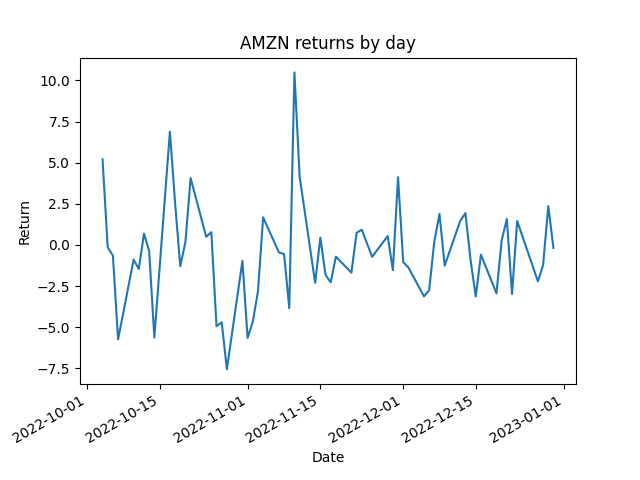
\includegraphics[width=.6\linewidth]{img/AMZN_daily_return.png}
    \caption{Stacionari laiko eilutė}
    \label{fig:sub1}
  \end{subfigure}%
  \begin{subfigure}{.5\textwidth}
    \centering
    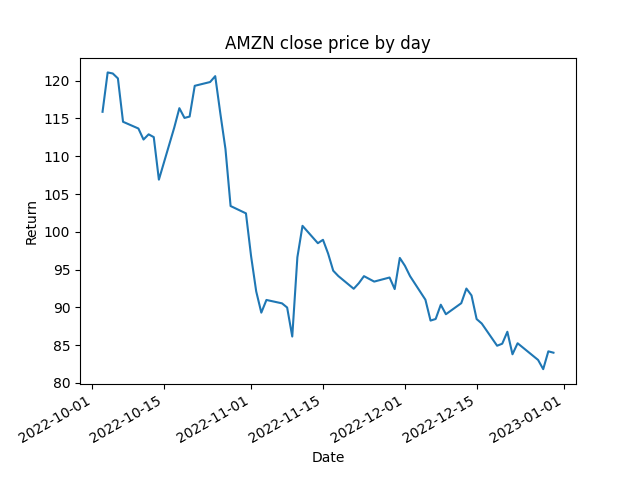
\includegraphics[width=.6\linewidth]{img/AMZN_daily_close.png}
    \caption{Nestacionari}
    \label{fig:sub2}
  \end{subfigure}
  \caption{Stacionari ir nestacionari laiko eilutė}
  \label{fig:test}
\end{figure}

Grafai parodantys skirtumą tarp stacionarios ir nestacionarios laiko eilutės. Grafuose naudojama "Amazon" kompanijos (NASDAQ: AMZN) akcijos duomenys gauti iš "Yahoo Finance" 
naudojant Python API\cite{yfinance}. Pirmajame (stacionariame) grafe yra pavaizduota kiekvienos dienos grąža investuojant į AMZN akciją trijų mėnesių laikotarpyje. 
Stacionarumas matomas ir vizualiai - vidurkis imtyje išlieka panašus, centruojasi ties 0, taip pat
% Variacija parodo kaip toli yra išsiskirste skaičiai imtyje, tai stacionariu atveju, nuo nulio atrodo visi panašų range turi. Variacija != standard deviation
% Kovariacija parodo kaip du kintamieji yra susije (teigiamai jei abu keičiasi vienodai arba negiamai jei keičaisi skirtinga kryptimi), čia svarbu kad ji išliktu vienoda (0 - nera rysio)
variacija ir kovariacija yra panašūs visuose taškuose. Antrame grafe yra pavaizduota tos pačios akcijos uždarymo kaina tokiame pat laikotarpyje. 
Nestacionarumas matomas ir vizualiai, kadangi yra akivaizdi tendencija žemyn. Šiuos teiginius patvirtina ir ADF testas. % Do I need to cite? 

% sources!!!!!!!
% later after introducing AR models?
% ACF : galima prieiti prie koreliacijos dviem budais S_t-2 -> S_t (tiesiogai) arba S_t-2 -> S_t-1 -> S_t (per visas reiksmes). ACF pasako 
% PACF: rupi TIK tiesiogine reiksme corr(2)? : S_t-2 -> S_t (kaip reiksme pries du men itakoja reiksme dabar) hence the naming PARTIAL
% ACF: is just pearson correlation with x/y data set where x: s_t-2 and y: s_t
% PACF: regression model.
\subsection {ACF ir PACF}
Autokoreliacijos funkcija (ACF) (angl. autocorrelation function) ir dalinė autokoreliacijos funkcija (PACF) (angl. partial autocorrelation function) naudojamos analizuoti laiko eilutes,
padedančios suprasti autokoreliacija duomenų rinkinyje. Pritaikant ACF bei PACF galima lengviau parinkti ARMA(p, q) ir ARIMA(p, d, q) modelių pradines reikšmes \cite{abu2017autoregressive}.
% boldify parameters?
Ženkliai didesnės reikšmės, pritaikius ACF laiko eilutei su tam tikru lagu, parodo optimalias ARMA ir ARIMA modelių slankaus vidurkio laipsnio (q) reikšmes. 
PACF tokiu pat būdu nurodo p - autoregresinio parametro reikšmę. 
%table of acf or pacf?

% There are a few things you can try to improve the test:
% try using a different test for stationarity, such as the Kwiatkowski-Phillips-Schmidt-Shin (KPSS) test or the Phillips-Perron (PP) test.
% try differencing the data to remove any trend or seasonality. This can help to stabilize the variance of the data and make it more stationary.
% try applying a transformation to the data, such as taking the log of the data, to stabilize the variance and make the data more stationary.
% try using more data in the test. A larger sample size may provide more accurate results.
% try using a longer time period for the test. This can provide a more accurate assessment of stationarity, as it takes into account any long-term trends or seasonality in the data.
\subsection{ADF testas}
ADF (Angl. Augmented Dickey-Fuller) testas nustato ar laiko eilutė yra stacionari. Tai yra dažnai naudojamas įrankis analizuojant laiko eilutės ir jų algoritmais, kurie tikisi stacionarių 
duomenų\cite{chi2018stock}. Stacionariai laiko eilutėje privaloma atmesti nulinę hipotezę tam tikrame užtikrintumo intervale. 
Jeigu ADF testo absoliuti statistinė vertė yra daugiau už kritinę vertę, nulinę hipotezę yra atmetama ir ši laiko eilutė yra stacionari.
pritaikius ADF testą{\cite{seabold2010statsmodels}} AMZN akcijų duomenims (\textbf{1 pav.}) gauti rezultatai:

% p reiksme, alfa reiksmingumo lygis
\begin{tabularx}{\linewidth}{|X|X|X|X|X|X|}
  \hline
  \textbf{Time Series} & \textbf{ADF Statistic} & \textbf{p-value} & \textbf{1\% Critical Value} & \textbf{5\% Critical Value} & \textbf{10\% Critical Value} \\ \hline
  Daily Returns        & -7.087727              & 0.000000         & -3.542                      & -2.910                      & -2.593                       \\ \hline
  Daily Close Price    & -1.640623              & 0.461935         & -3.542                      & -2.910                      & -2.593                       \\ \hline
\end{tabularx}

\vspace{10pt}
Pagal šiuos rezultatus
\begin{itemize}
  \item ADF statistika yra skaičius, kuris lyginamas su kritinėmis vertėmis iš lentelės (skirtingais lygiais), kad būtų nuspręsta, ar atmesti ar priimti nulio hipotezę apie stacionarumą.
  \item Pirmu atveju ADF statistika dienos grąžoms yra -7.087727, kuri mažesnė, nei kritinė vertė -3.542 1\% lygyje. Todėl nulinė hipotezė yra atmesta ir laiko seka laikoma stacionaria.
  \item Antru atveju ADF statistika dienos uždarymo kainoms yra -1.640623, kuris yra nemažesnė, nei kritinė vertė -3.542 1\% lygyje. Todėl nulio hipotezė nėra atmesta ir laiko seka laikoma nestacionari.
\end{itemize}

% autoregression crypto currency predict
% ar, ar-abs, arima, arfima, sarima
\section{Autoregresiniai modeliai}
Vienas iš būdų analizuoti laiko eilutės yra autoregresija ir ją naudojantis modeliai. Egzistuoja ne vienas autoregresija naudojantis modelis. 
Populiarusi ir dažniausiai sutinkami modeliai yra ARMA(p, q) ir ARIMA(p, d, q).
Šie modeliai taip pat naudojasi anksčiau nepaminėtu MA modeliu kuris yra slankaus vidurkio modelis (angl. MA - moving average).
Taip pat yra SARIMA, SARFIMA ir kitų modelių, turinčių savo specifinius panaudjimo atvejus. 
Toliau apžvelgsime detaliau autoregresinius modelius ir kaip jie galėtų būti panaudoti iškeltiems užduotims šiame darbe spręsti.

\subsection{AR modelis}
AR (angl. autoregressive) modelis remiasi tik praeities duomenimis, kad nuspėti kintamojo reikšme ateityje, ieškoma ar pastebimas pasikartojantis
modelis, kuris padėtų tiksliau nuspėti dydį ateityje\cite{chi2018stock}. Šis modelis dar dažnai vadinamas ARp modeliu, nes naudojamas kintamasis "p", nusakantis kiek praeiteis reikšmių 
iš laiko periodo norima naudoti. Laikant, kad kintamasis X yra laiko eilutės kintamasis AR(p) modelio formulė gali atrodyti taip: 
\[X_{t} = \Phi _{1}X_{t-1}+\epsilon_{t} \]

%\cite{chi2018stock} naudojami AR, MA ir ARMA modelio formulėms
${X_t}$ - stacionari laiko eilutė, $\Phi$ - AR modelio koeficientas, P - AR modelio laipsnis, $ \epsilon_{t} $ - AR modelio paklaida.

\subsection {MA modelis}
Toliau tyrinėjami autoregresyvieji modeliai susideda iš dar vienos dalies - Slankaus vidurkio - MA (angl. Moving average). Slenkančio vidurkio dabartinė
reikšmė tiesiškai priklauso nuo dabartines ir praeitų reikšmių. Žymėjimas MA(q) reiškia q laipsnio slenkamajį vidurkį, kurio formulę atrodo taip:  
\[X_{t} = \epsilon_{t} - \sum_{i=1}^{q}\theta_{i}  \epsilon_{t-i}\]

${X_t}$ - stacionari laiko eilutė, q - MA modelio laipsnis, ${\epsilon_t}$ - MA modelio paklaida.

\subsection {ARMA modelis}
ARMA (angl. autorogressive moving average) modelis yra autoregresyviaus ir slankaus vidurkio modelio junginys. Modelis dažnai žymimas
kaip ARMA(p, q), kur p yra AR laipsnis, o q yra MA laispnis. Pirmą kartą sujungtas 1938 mokslininko Herman Wold, jis pastebėjo jog ARMA modelis gal apimti 
dideles stacionarias laiko eilutes, kai yra tinkamai nurodytas p laipsnis ir q laipsnis\cite{makridakis1997arma}. Taip pat reikia pabrėžti, 
jog ARMA(0, q) = MA(q) ir ARMA(p, 0) = AR(p) Reiškia, jog Xt eilutė gali būti modeliuojama kaip kombinacija praeities $x_{t}$ reikšmių ir/arba praeities $e_{t}$ klaidų:
\[X_{t} = \phi_{1}x_{t-1} + \phi_{2}x_{t-2} + ... + \phi_{p}x_{t-p} + e_{t} - \theta_{1}e_{t-1} - \theta_{2}e_{t-2} - ... - \theta_{q}e_{t-q}\]


\subsection {ARIMA modelis}
ARIMA (angl. autoregressive integrated moving average) modelis yra paplitęs nuo 1970-ųjų iki šių dienų. Modelio pavadinimo šifravimas
pažodžiui: AR - Autoregresinis modelis, I - Integracija (Diferencijavimas), atsižvelgiama į duomenų tendenciją, MA - (Moving average) slankusis vidurkis.
AR ir MA yra atskiri modeliai, kurie gali būti naudojami paprastesnei laiko eilučiu analizei. Šio modelio privalumas, jog jis sujungia AR ir MA naudojimą kartu su
diferencijavimu, kuris suteikia galimybė giliau analizuoti laiko eilutes. Diferencijavimo dalis turimus duomenis padeda paversti į stacionarius, 
kurie yra reikalingi korektiškam modelio veikimui. Diferencijavimas vyksta baigtinį kartų skaičių, jog būtų pasiekta beveik-validi stacionari būseną. 
Kitais žodžiais ARIMA yra ekvivalentus ARMA modelis tiem patiems MA ir AR laipsniams \cite{hua2020bitcoin}. Taigi ARIMA modelis yra paremtas ARMA modeliu. 
Pagrindinis skirtumas tarp šių modelių yra tas, jog ARIMA konvertuoja nestacionarius duomenis į stacionarius prieš dirbant su jais. Modelio tipas yra 
klasifikuojamas kaip ARIMA(p,d,q), kur p - autoregresyvoji dalis, d - integravimo (diferencijavimo) dalis, q - slenkančio vidurkio dalis. Visos ARIMA modelio
reikšmės yra neneigiami sveikieji skaičiai \cite{mondal2014study}.

% Not sure about this
% dažniausiai negalima naudoti šiame kontekste
Dažniausiai yra 3 žingsniai naudoti ARIMA modelį:
\begin{enumerate}
  \item Duomenų surinkimas ir verifikavimas - tikriname ar gauti duomenys yra stacionarūs ir ieškome sezoniškumo.
  \item Diferencijavimas - vertimas laiko eilutę į stacionarią.
  \item Prognozavimas naudojant ARIMA modelį - dažniausias taikomas ARIMA modelis yra ARIMA(1,1,0)
\end{enumerate}

\subsection {SARIMA modelis}
SARIMA (angl. seasonal autoregressive integrated moving average) modelis yra ARIMA modelio išplėtimas turintis vieną papildomą savybę - sezoniškumą\cite{carl2020ethereum}. 
Pastebėjus, jog periodiškai kartojasi rezultatai laiko eilutėse, galima taikyti šį modelį. Geras ir paprastas pavyzdys, prekyba šventiniu laikotarpiu - kalėdos.
Prekybos centruose, tuo metu padidėja prekybą, tačiau kitą mėnesį ženkliai sumažėja. Spartus sumažėjimas nereiškia, jog prekybai yra didėlės problemos ir reikia pokyčių.
Tai dažniausiai yra žmonių poilsis nuo pirkinių po šventinio laikotarpio. šis modelis pastebi panašius sezoniškai atsitinkančius įvykius, juos atpažįsta ir pritaiko naudojant
ankščiau minėtą ARIMA modelį.

SARIMA galima išreikšti kaip ARIMA(p,d,q)(P,D,Q)[S], kur p,d,q standartiniai ARIMA modelio parametrai, o P - sezoniškumo autoregresivumo laipsnis,
D - sezoniškumo diferencijavimo laipsnis, Q - sezoniškumo slankiojo vidurkio laipsnis ir S - sezoniškumo ciklio ilgis. 

%what abous AR ABS? autoregressive - asset backed security
% autoregression crypto currency predict
%\subsection(Auto regressive - ABS)% atskirti trumpos atminties ir ilgos taminties modelius?
\subsection {ARFIMA modelis}
ARFIMA (angl. autoregressive fractionally integrated moving average) modelis yra ARIMA modelio išplėtimas.
Šis modelis apibendrina autoregresyvų integruotą slankiojo vidurkio (ARIMA) modelį su sveikaisiais integracijos laipsniais.
Parametrizavimas sujungia autoregresyvų slankiojo vidurkio (ARMA) modelį, kuris yra plačiai naudojamas trumpos atminties procesu, taip 
patampant ilgos atminties procesu. ARFIMA tinka analyzuoti toliau į priekį lyginant su ARIMA trumpos atminties procesu \cite{samimi2009long}.

% parašyti kas tokie tiksliai yra p ir q
Atliekamos trys procedūros prieš pradedant naudoti ARFIMA(p,d,q) modelį:
Testuojama laiko eilutės ilgos atminties savybės ir nustatoma trupmeninio diferencijavimo parametrą d.
Trupmeniškai diferencijuojama laiko eilutė, ko pasekoje gaunamas ARMA procesas.
Nustatomi kiti du ARFIMA modelio parametrai p ir q.
% šis modelis iš esmės 

\section{Prognozės}
Prognozuoti kriptovaliutas naudojami duomenys iš Binance API\cite{binanceKlines}, imant 2022 metų gruodžio mėnesio 15 minučių intervalo duomenis.
Prognozavimui naudojamas 90 procentų dumomenų rinkinio dydis modelio pradiniam modelio apmokymui, kitus 10\% bandoma prognozuoti po vieną reikšmę cikle kiekvieną
kartą iš naujo apmokus modelį su tikra reikšmę. Tikrinimui naudosime MSE ir MAPE paklaidas.
Kadangi kriptovaliutų duomenys nėra stacionarūs, jiem visiem iškarto tenka taikyti diferencijavimą, todėl pradėta nuo ARIMA modelio nes jį naudoja ir AR
ir MA modelį ir iškarto pritaiko diferencijavimą, taip galėdamas dirbti ir su nestacionariais duomenimis. ARFIMA modelis šiuo atveju taip pat nėra aktualus,
nes prognozuojamas laiko tarpas yra viena reikšmė į ateitį.
\subsection{ARIMA}
Prognozuojant naudojamos ARIMA pagalbinės bibliotekos\cite{seabold2010statsmodels} bei heuristins $AUTO_ARIMA$ algoritmas\cite{pmdarima} padedantis nustatyti geriausius ARIMA parametrus konkrečiam duomenų rinkiniui.

\begin{figure}[H]
  \centering
  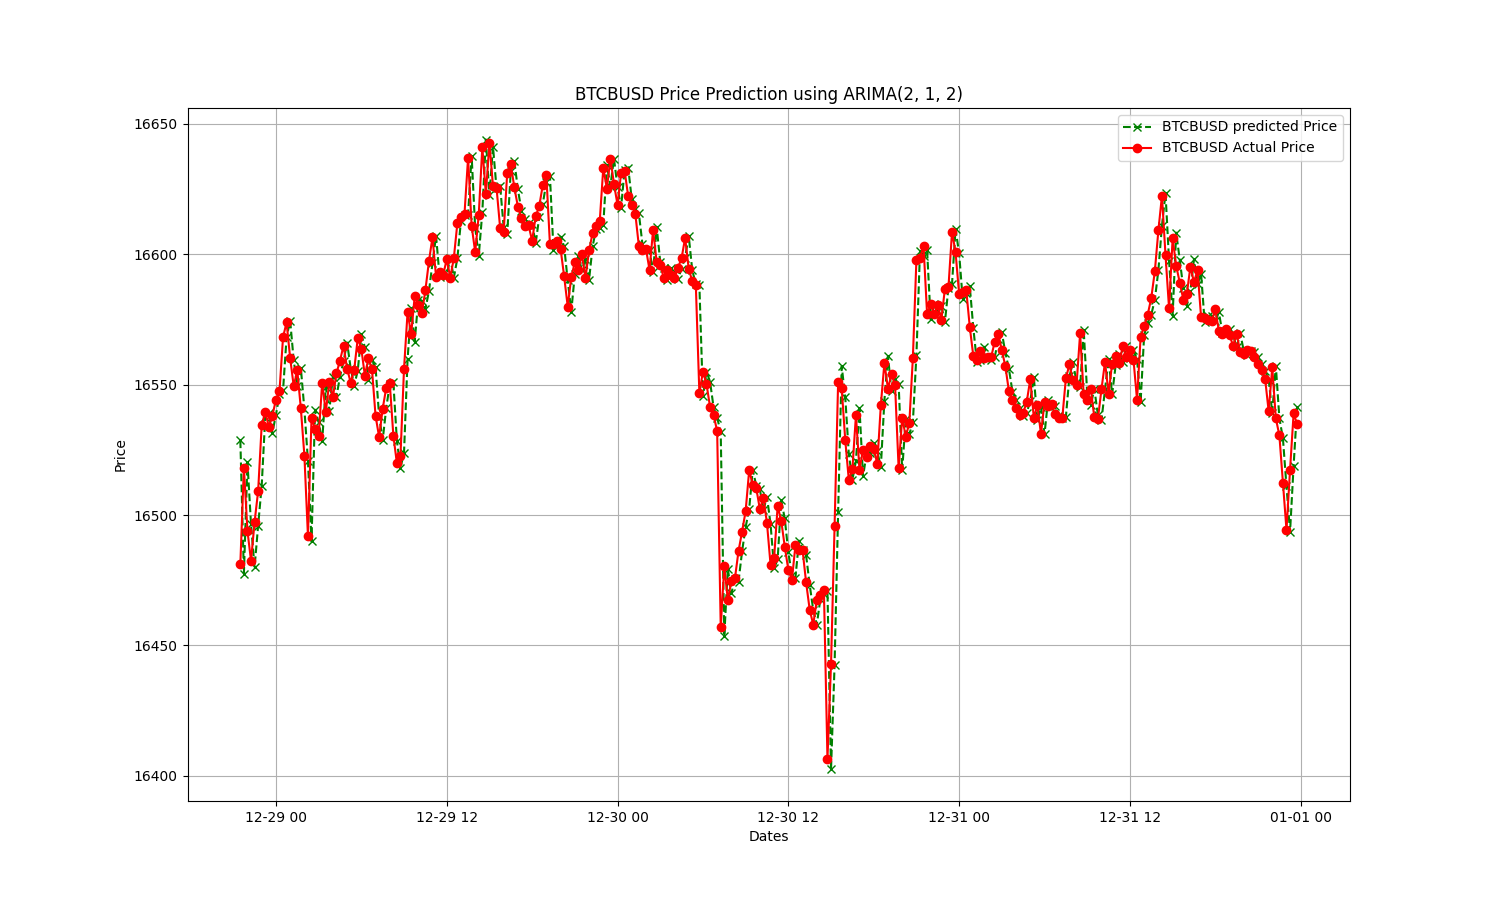
\includegraphics[scale=0.35]{img/BTCBUSD_15m_dec_final.png}
  \caption{BTCBUSD poros prognozės ir tikrų verčių grafas}
  \label{fig:btcbusd_results}
\end{figure}

BTCBUSD Gautos paklaidos:
\textbf{MSE}: 210.83
\textbf{MAPE}: 0.061 \%


\begin{figure}[H]
  \centering
  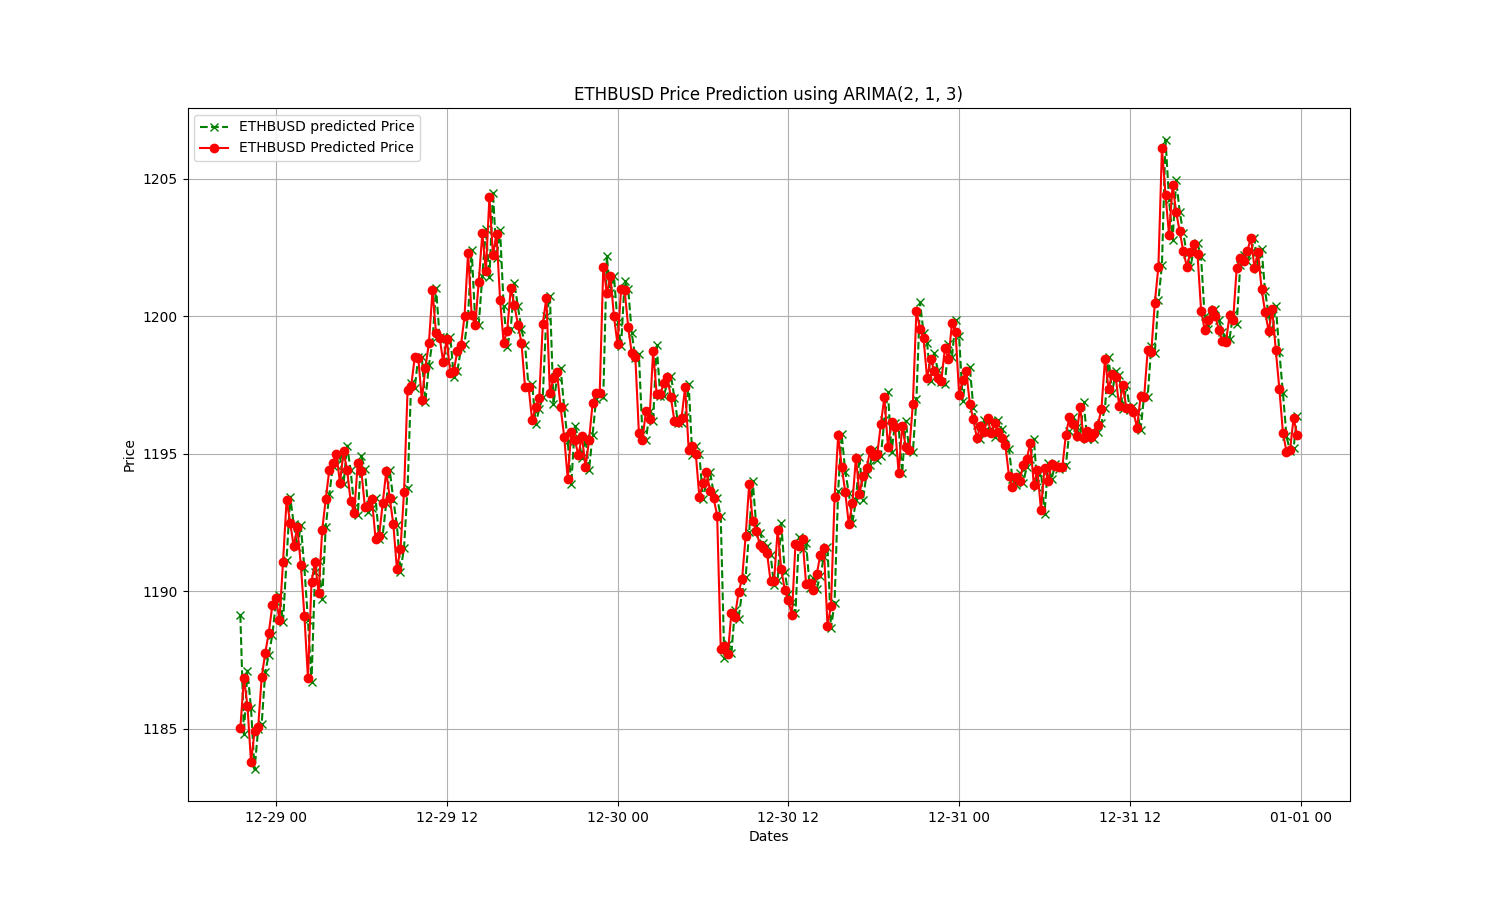
\includegraphics[scale=0.35]{img/ETHBUSD_15m_dec_final.png}
  \caption{ETHBUSD poros prognozės ir tikrų verčių grafas}
  \label{fig:ethbusd_results}
\end{figure}

ETHBUSD Gautos paklaidos:
\textbf{MSE}: 1.69
\textbf{MAPE}: 0.082 \%

\subsection{SARIMA}
SARIMA modeliui parametrams parinkti taip pat naudojama $AUTO_ARIMA$ algoritmas, sezoniškumo intervalas naudojamas 4, bandoma pamatyti ar atsiranda
sezoniškumas kiekvieną valandą, nes duomenų intervalas yra 15min.

\begin{figure}[H]
  \centering
  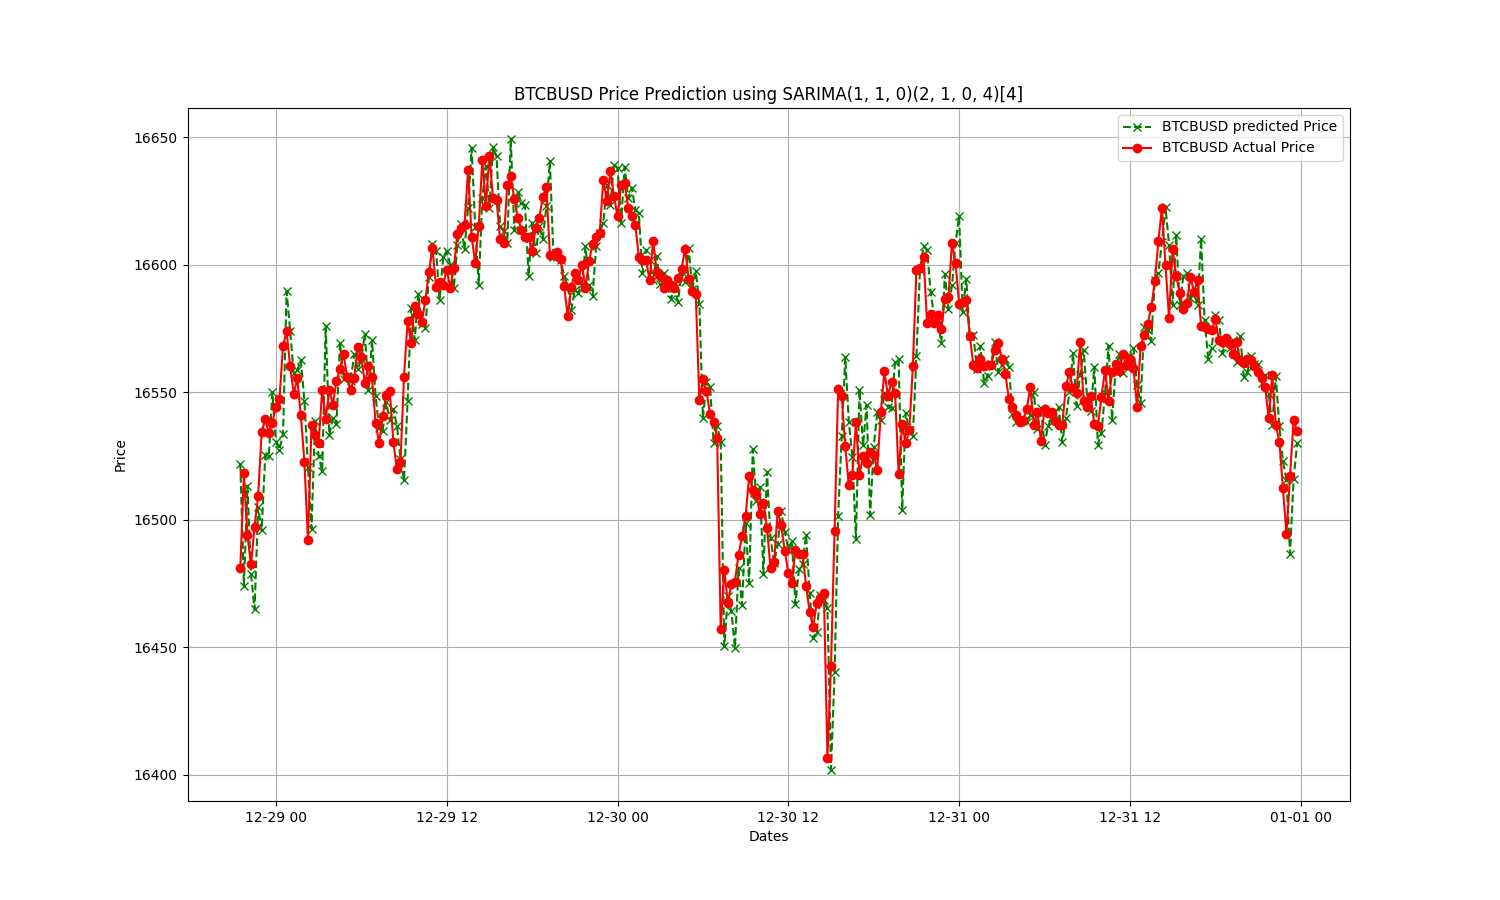
\includegraphics[scale=0.35]{img/btcbusd_sarim_full.png}
  \caption{BTCBUSD poros prognozės ir tikrų verčių grafas}
  \label{fig:btcbusd_sarima_results}
\end{figure}

BTCBUSD Gautos paklaidos:
\textbf{MSE}: 288.87
\textbf{MAPE}: 00.07\%

\begin{figure}[H]
  \centering
  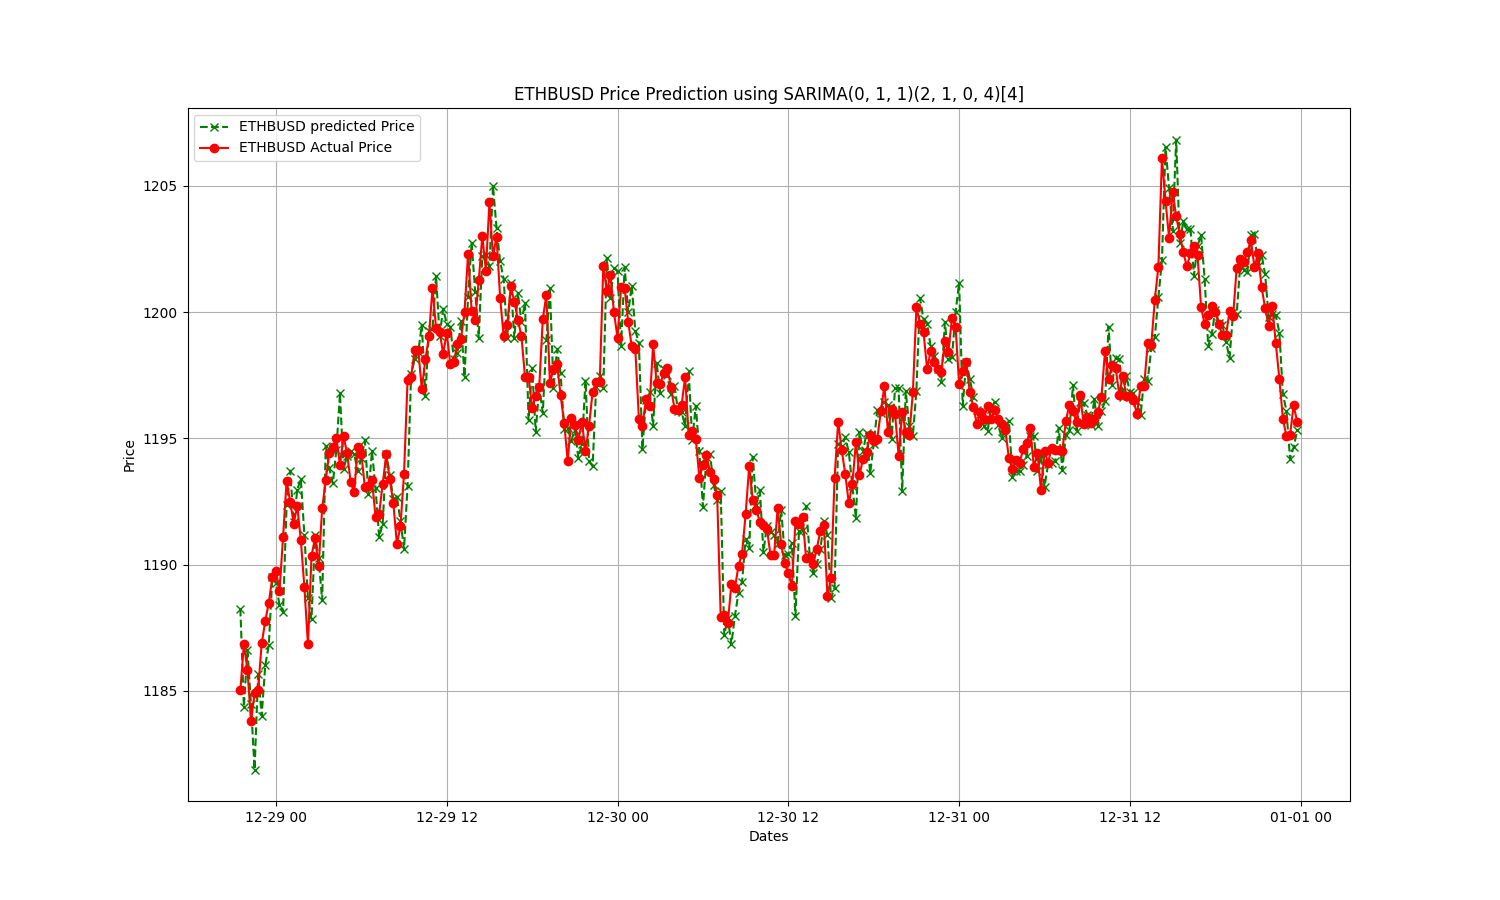
\includegraphics[scale=0.35]{img/ethbusd_sarima_full.png}
  \caption{ETHBUSD poros prognozės ir tikrų verčių grafas}
  \label{fig:ethbusd_sarima_results}
\end{figure}


ETHBUSD SARIMA Gautos paklaidos:
\textbf{MSE}: 2.306
\textbf{MAPE}: 00.09\%

\vspace{20pt}

\begin{table}[h]
  \centering
  \caption{MSE ir MAPE palyginimas ETHBUSD ir BTCBUSD kriptovaliutų poromis}
  \begin{tabularx}{\linewidth}{|X|X|X|}
    \hline
    \textbf{Model} & \textbf{MSE} & \textbf{MAPE} \\ \hline
    ETHBUSD SARIMA & 2.306        & 0.09\%        \\ \hline
    ETHBUSD ARIMA  & 1.69         & 0.082\%       \\ \hline
    BTCBUSD SARIMA & 288.87       & 0.07\%        \\ \hline
    BTCBUSD ARIMA  & 210.83       & 0.061\%       \\ \hline
  \end{tabularx}
\end{table}

\section{Rezultatai ir išvados}
Atlikta mokslinė analizė, literatūros apžvalga, kurios dėka pavyko aiškiau suprasti statistinius modelius ir kriptovaliutų rinką, bei naudojamus įrankius.
Palyginti autoregresiniai modeliai ir kuo jie skiriasi. Padėti pamatai kurti robotui, kuris galėtų implementuoti reikalinga strategiją, susipažinta kokią
darbinę aplinką teks naudoti, python ir python-binance biblioteką.

Matome, kad prognozuojant kiekviename žingsnyje naują 15m intervalu valiutos kainą, visumoje absoliutus paklaidos procentas gaunasi gana mažas, tačiau
nereikia pamiršti, jog kaina per 15m pasikeičia neperdaugiausiai. Rezultatai neblogi, bet tai nereiškia, kad galima taikyti lošimo taktika ir iškarto išlošti daug pinigų,
jei bus keičiamasi tuo pačiu 15min dažniu šie procentai greit susideda ir reikia apmastyti lošimo strategiją.

% Išvadose ir pasiūlymuose, nekartojant atskirų dalių apibendrinimų,
% suformuluojamos svarbiausios darbo išvados, rekomendacijos bei pasiūlymai.
% \sectionnonum{Išvados}
\vspace{10pt}
Taigi galima kurti robotą kuris prekiauja remiantis autoregresiniais modeliais.
\begin{itemize}
  \item Kadangi kainos nėra stacionarus duomneys negalima naudoti paprastesnių AR, ARMA modelių.
  \item Geriausi rezultatai gaunami naudojant ARIMA modelį nei SARIMA modelį;
  \item Paklaidos gaunasi gana mažos, todėl galima implementuoti norima strategija robotui lošti
\end{itemize}
Neišvengiama, jog tokiame trumpame darbe būtų aptartos visos įmanomos sritys ir atvejai, taigi tolimesnei tyrimo eigai pasiūlymas nagrinėti prognozuojamus modelius, 
kurie naudoja dirbtinį intelektą. Suprasti jų veikimą ir palyginti su standartiniais statistiniais prognozavimo būdais aptartais šiame darbe arba kitais nepaminėtais
prognozavimo modeliais (VAR, GARCH). Šiame darbe apsistojama ties kainų tendencijų prognozavimų, tolimesnė programos galima eiga būtų realizuoti pritaikyti konkrečias strategijas 
robotui lošėjui, kuris pagal gautas prognozes atlieka atitinkamą veiksmą.

\sectionnonum{Sąvokų apibrėžimai}
\textbf{API} - Aplikacijų programavimo sąsaja (angl. Application programming interface), tai sistemos suteikiama sąsaja, kuria galima naudotis norint pasiekti tos sistemos
funckionalumą ar apsikeisti duomenimis.

\textbf{Autoregresinis modelis} - Statistinis modelis yra autoregresinis, jei jis numato būsimas reikšmes pagal praeities reikšmes. Pavyzdžiui, autoregresinis modelis gali
siekti numatyti būsimas akcijų kainas, remiantis ankstesniais rezultatais.

\textbf{Euristinis algoritmas} - euristiniai algoritmai yra tokios intelektualios optimizavimo uždavinių sprendimo priemonės, kuriomis siekiama rasti aukštos
kokybės (bet nebūtinai optimalius) sprendinius per priimtiną laiką. Algoritmas negarantuoja, kad rastas sprendimas bus optimalus. \cite{misevivcius2009euristiniku}

\textbf{Kriptovaliuta} - Kriptovaliuta yra skaitmeninė arba virtuali valiuta, kuri yra apsaugota kriptografija, todėl beveik neįmanoma jos padirbti ar išleisti dvigubai.

\textbf{Kriptovaliutų pora} - Kriptovaliutų pora rinkoje yra naudojama prekiaujant. Kriptovaliutos yra susietos poromis, tad norint nusipirkt BTC valiutos pirmiausia reikia surasti 
galimus keitimo variantus, jei egzistuoja pora BTC/BUSD, galima nusipirkti BTC kriptovaliutos uz turimas BUSD valiutas. Dažnu atveju rinkoje pasidėjus ("FIAT") valiuta
prekybos rinką ją konvertuoją i panašių token valiuta kaip BUSD(us -regulated stablecoin), USDT (usd tether) ar BNB (binance coin)

\textbf{MSE} - Vidutinė kvadratinė paklaida, angl. (Mean squared error)

\textbf{MAPE} - Vidutinė  bsoliučioji paklaida išreikšta procentais, angl. (Mean absolute percentage error)

\printbibliography[heading=bibintoc] % Literatūros šaltiniai aprašomi
% bibliografija.bib faile. Šaltinių sąraše nurodoma panaudota literatūra,
% kitokie šaltiniai. Abėcėlės tvarka išdėstoma tik darbe panaudotų (cituotų,
% perfrazuotų ar bent paminėtų) mokslo leidinių, kitokių publikacijų
% bibliografiniai aprašai (šiuo punktu pasirūpina LaTeX). Aprašai pateikiami
% netransliteruoti.

\appendix  % Priedai
% Prieduose gali būti pateikiama pagalbinė, ypač darbo autoriaus savarankiškai
% parengta, medžiaga. Savarankiški priedai gali būti pateikiami kompiuterio
% diskelyje ar kompaktiniame diske. Priedai taip pat vadinami ir numeruojami.
% Tekstas su priedais siejamas nuorodomis (pvz.: \ref{img:mlp}).

\end{document}
